% This is "sig-alternate.tex" V2.1 April 2013
% This file should be compiled with V2.5 of "sig-alternate.cls" May 2012
%
% This example file demonstrates the use of the 'sig-alternate.cls'
% V2.5 LaTeX2e document class file. It is for those submitting
% articles to ACM Conference Proceedings WHO DO NOT WISH TO
% STRICTLY ADHERE TO THE SIGS (PUBS-BOARD-ENDORSED) STYLE.
% The 'sig-alternate.cls' file will produce a similar-looking,
% albeit, 'tighter' paper resulting in, invariably, fewer pages.
%
% ----------------------------------------------------------------------------------------------------------------
% This .tex file (and associated .cls V2.5) produces:
%       1) The Permission Statement
%       2) The Conference (location) Info information
%       3) The Copyright Line with ACM data
%       4) NO page numbers
%
% as against the acm_proc_article-sp.cls file which
% DOES NOT produce 1) thru' 3) above.
%
% Using 'sig-alternate.cls' you have control, however, from within
% the source .tex file, over both the CopyrightYear
% (defaulted to 200X) and the ACM Copyright Data
% (defaulted to X-XXXXX-XX-X/XX/XX).
% e.g.
% \CopyrightYear{2007} will cause 2007 to appear in the copyright line.
% \crdata{0-12345-67-8/90/12} will cause 0-12345-67-8/90/12 to appear in the copyright line.
%
% ---------------------------------------------------------------------------------------------------------------
% This .tex source is an example which *does* use
% the .bib file (from which the .bbl file % is produced).
% REMEMBER HOWEVER: After having produced the .bbl file,
% and prior to final submission, you *NEED* to 'insert'
% your .bbl file into your source .tex file so as to provide
% ONE 'self-contained' source file.
%
% ================= IF YOU HAVE QUESTIONS =======================
% Questions regarding the SIGS styles, SIGS policies and
% procedures, Conferences etc. should be sent to
% Adrienne Griscti (griscti@acm.org)
%
% Technical questions _only_ to
% Gerald Murray (murray@hq.acm.org)
% ===============================================================
%
% For tracking purposes - this is V2.0 - May 2012
\usepackage{subcaption}
\usepackage{subfig}
\documentclass{sig-alternate-05-2015}


\newlength{\blackoutwidth}
\newcommand{\blackout}[1]
{%necessary comment
  \settowidth{\blackoutwidth}{#1}%necessary comment
  \rule[-0.3em]{\blackoutwidth}{1.125em}%necessary comment
}


\begin{document}

% Copyright
\setcopyright{acmcopyright}
%\setcopyright{acmlicensed}
%\setcopyright{rightsretained}
%\setcopyright{usgov}
%\setcopyright{usgovmixed}
%\setcopyright{cagov}
%\setcopyright{cagovmixed}


% DOI
\doi{10.475/123_4}

% ISBN
\isbn{123-4567-24-567/08/06}

%Conference
\conferenceinfo{PLDI '13}{June 16--19, 2013, Seattle, WA, USA}

\acmPrice{\$15.00}

%
% --- Author Metadata here ---
\conferenceinfo{WOODSTOCK}{'97 El Paso, Texas USA}
%\CopyrightYear{2007} % Allows default copyright year (20XX) to be over-ridden - IF NEED BE.
%\crdata{0-12345-67-8/90/01}  % Allows default copyright data (0-89791-88-6/97/05) to be over-ridden - IF NEED BE.
% --- End of Author Metadata ---

\title{A Metric for Hand Comfort/Discomford Evaluation} 
\subtitle{Towards Expressivity in Spatial Control}
%\titlenote{(Produces the permission block, and
%copyright information). For use with
%SIG-ALTERNATE.CLS. Supported by ACM.}}
%\subtitle{[Extended Abstract]
%\titlenote{A full version of this paper is available as
%\textit{Author's Guide to Preparing ACM SIG Proceedings Using
%\LaTeX$2_\epsilon$\ and BibTeX} at
%\texttt{www.acm.org/eaddress.htm}}}
%
% You need the command \numberofauthors to handle the 'placement
% and alignment' of the authors beneath the title.
%
% For aesthetic reasons, we recommend 'three authors at a time'
% i.e. three 'name/affiliation blocks' be placed beneath the title.
%
% NOTE: You are NOT restricted in how many 'rows' of
% "name/affiliations" may appear. We just ask that you restrict
% the number of 'columns' to three.
%
% Because of the available 'opening page real-estate'
% we ask you to refrain from putting more than six authors
% (two rows with three columns) beneath the article title.
% More than six makes the first-page appear very cluttered indeed.
%
% Use the \alignauthor commands to handle the names
% and affiliations for an 'aesthetic maximum' of six authors.
% Add names, affiliations, addresses for
% the seventh etc. author(s) as the argument for the
% \additionalauthors command.
% These 'additional authors' will be output/set for you
% without further effort on your part as the last section in
% the body of your article BEFORE References or any Appendices.




%\numberofauthors{0} %  in this sample file, there are a *total*
% of EIGHT authors. SIX appear on the 'first-page' (for formatting
% reasons) and the remaining two appear in the \additionalauthors section.
%
%\author{
% You can go ahead and credit any number of authors here,
% e.g. one 'row of three' or two rows (consisting of one row of three
% and a second row of one, two or three).
%
% The command \alignauthor (no curly braces needed) should
% precede each author name, affiliation/snail-mail address and
% e-mail address. Additionally, tag each line of
% affiliation/address with \affaddr, and tag the
% e-mail address with \email.
%
% 1st. author
%\alignauthor
%\blackout{Jonas Mayer}\\
%       \affaddr{\blackout{Technical University of Munich}}\\
%       \affaddr{\blackout{Arcisstra\ss e 21}}\\
%       \affaddr{\blackout{Munich, Germany}}\\
%       \email{\blackout{ga97qic@mytum.de}}
% 2nd. author
%\alignauthor
%\blackout{Nicholas Katzakis}\\
%       \affaddr{\blackout{Technical University of Munich}}\\
%       \affaddr{\blackout{Arcisstra\ss e 21}}\\
%       \affaddr{\blackout{Munich, Germany}}\\
%       \email{\blackout{niko@tum.de}}
}
% There's nothing stopping you putting the seventh, eighth, etc.
% author on the opening page (as the 'third row') but we ask,
% for aesthetic reasons that you place these 'additional authors'
% in the \additional authors block, viz.
% Just remember to make sure that the TOTAL number of authors
% is the number that will appear on the first page PLUS the
% number that will appear in the \additionalauthors section.

\maketitle


\begin{abstract}
In this paper a straightforward metric for quick comfort and discomfort evaluation of non-resting hand postures is proposed, which is improved using data from user studies. Comparing user ratings with the metric indicates the metric to be a fitting extrapolating model for perceived comfort and discomfort. Our results also indicate the affect of hand comfort and discomfort on precision and performance.
\end{abstract}


%
% The code below should be generated by the tool at
% http://dl.acm.org/ccs.cfm
% Please copy and paste the code instead of the example below. 
%
\begin{CCSXML}
<ccs2012>
<concept>
<concept_id>10003120.10003123.10011758</concept_id>
<concept_desc>Human-centered computing~Interaction design theory, concepts and paradigms</concept_desc>
<concept_significance>500</concept_significance>
</concept>
</ccs2012>
\end{CCSXML}

\ccsdesc[500]{Human-centered computing~Interaction design theory, concepts and paradigms}


\begin{figure}
\centering
\includegraphics[width=8.45cm]{Robot}
\vspace{-20pt}
\caption{Controlling a Robot using Hand Postures}
\label{fig:Robot}
\vspace{-5pt}
\end{figure}

%
% End generated code
%

%
%  Use this command to print the description
%
\printccsdesc

% We no longer use \terms command
%\terms{Theory}

\keywords{comfort/discomfort metric, hand posture}

\section{Introduction}

In a traditional desktop computer environment, there exist a number of different standardized interfaces for human-computer interaction using a mouse, keyboard and monitor. This allows the user to 
complete a variety of tasks effectively and efficiently by providing sets of shortcuts and macros. 

However, in contexts such as virtual reality and robotics traditional input methods are often not suitable for the tasks environment. Therefore both speech as well as hand gestures and postures are common interaction concepts. While speech interaction is often struggling with its limited powerfulness for spatial navigation, postures in particular are highly useful for such tasks (Figure \ref{fig:Robot}). The main challenge for gestures and postures has been fighting physical forces that cause fatigue or discomfort, which limit user experience as well as precision and performance, as indicated by Short et al. \cite{short1999precision}. Even though comfort and discomfort are often taken into consideration by designers, there are only a few quantitative evaluation methods\cite{naddeo2015proposal}.

This work is meant to support the creation and evaluation of a hand posture catalog for effective and efficient human-robot interaction. For that we propose a hand posture comfort/discomfort metric that allows for quick objective hand posture evaluation. State of the art comfort/discomfort models were combined with current hand anatomy and ergonomics knowledge to create models for hand comfort and discomfort. Based on our model we created a naive metric, which we improved in a second step using data from a user study. Finally another user study was used to validate our metric and to show the impact of comfort and discomfort on performance in a hand pointing task.

We will first explain the theoretical basis of our comfort/discomfort model, before deriving our naive metric. After that we will explain the methodology used for optimizing and validating the metric as well as for showing the metric's influence on performance in a pointing task. Finally, the results will be analyzed and discussed, before our findings are evaluated and put in a greater context.


\section{Hand Posture Comfort/Discomfort Metric}
The structure of the metric proposed is based on current ergonomics models \cite{vink2012editorial}. These define comfort as a ``pleasant state or relaxed feeling of a human being" mostly caused by subjective impressions and expectations and discomfort as ``an unpleasant state of the human body" resulting from physical stress. Using this information and knowledge of the human hand anatomy, we broke down human hand comfort and discomfort in a non-resting hand into the following four components, which will be explained in the following sections: 

\begin{itemize}
	\item Deviation from Range of Rest Posture (RRP)
	\item Inter Finger Angles (IFA)
	\item Finger Hyperextension (HE)
	\item Finger Abduction (FA)
\end{itemize}

For the computation of our metric we used an angle based hand model, similar to the model described by Su et al. \cite{su1994logical}, as it makes reading joint angles trivial. Instead of the full 23 degrees of freedom, described by LaViola \cite{laviola1999survey}, we used a simplified model that neglects the MCC (metacarpocarpal joint) (Figure \ref{fig:handAnatomyTotal}) of the fourth and fifth digit. The simplification was applied because the \textbf{Leap} uses the same model and due to the MCC generally not being noticeable to influence hand postures.

The 21 DOF angle based hand model was furthermore simply handled as a vector of 21 \texttt{float}s. 

\begin{figure}
\centering
\begin{subfigure}
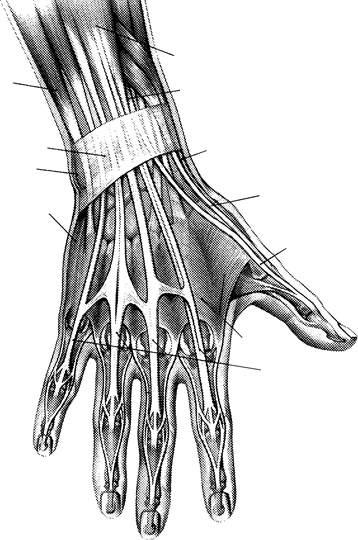
\includegraphics[width=4cm]{Handanatomy2}
\end{subfigure}
\begin{subfigure}
\includegraphics[width=4cm]{handanatomy}
\end{subfigure}
\caption{Hand Anatomy}
\label{fig:handAnatomyTotal}
\end{figure}

\subsection{Deviation from Range of Rest Posture}

%rest on supports
\textbf{Range of Rest Posture (RRP)} is a range of angles for an articular joint\footnote{The word ``articular joint" refers to the joints in the human body.}, where the joint "can be considered statistically in rest"\cite{apostolico2014postural}. The resulting relaxation of muscles and tendons creates a maximum of comfort in this particular joint. In our case, we considered the non-resting human hand to have a particular RRP for each finger joint, when the palm faces downwards. The combination of the latter results in a range of relaxed hand postures where the comfort is maximized. 

For articular joints perceived comfort decreases when deviating from the RRP. It minimizes at the bounds of the natural range of motion. Applying this to the whole hand leads to the conclusion, that hand posture comfort can be evaluated by adding up the individual joint angle distances to the RRP. \cite{naddeo2015proposal}

In our implementation the RRP was represented by a set of 50 relaxed hand postures recorded with the Leap. The metric \textbf{RRP(x)} was simply computed by calculating the minimum euclidean distance of a hand denoted as ``x" to the RRP set.
For simplicity we supposed the comfort to linearly decrease with distance to the RRP in our metric.

\subsection{The Inter Finger Angles}

The hand has a very compact and highly connected system of muscles and tendons that limits the individual movement of fingers \ref{fig:handAnatomyTotal}.
The fingers, excluding the thumb, share \textsl{most} of their flexor and extendor muscles, however minor individual flexion and extension (Figure \ref{fig:hyperabduction}) of adjacent fingers is still possible due to finger tendons originating from different areas of the muscles. In the case of the EDC (\textit{Extensor digitorum communis}) (Figure \ref{fig:handAnatomyTotal}) the finger tendons are even interconnected on the back of the hand. 

Therefore hand postures with high bending differences of adjacent fingers should lead to stress of tendons and muscles, as well as cognitive stress. This should minimize comfort and increase perceived discomfort.

The \textbf{inter finger angle component} \textbf{IFA(x)} was computed by first summing up the flexion/extension angles of MCP (\textit{metacarpophalangeal}), PIP(\textit{proximal interphalangeal}) and DIP (\textit{distal interphalangeal}) joints (Figure \ref{fig:handAnatomyTotal}) for each finger and adding up the differences in total bending of adjacent fingers (3 values). In order to compensate anatomical differences of the fingers, mostly affecting the ring finger, we added a ring finger bonus consisting of the difference of the ring finger's bending to both of his neighbors multiplied with an estimated weighting coefficient. The importance of this differentiation can be seen in when extending the index finger from a closed fist as opposed to extending the ring finger. 

\begin{figure}[b]
\centering
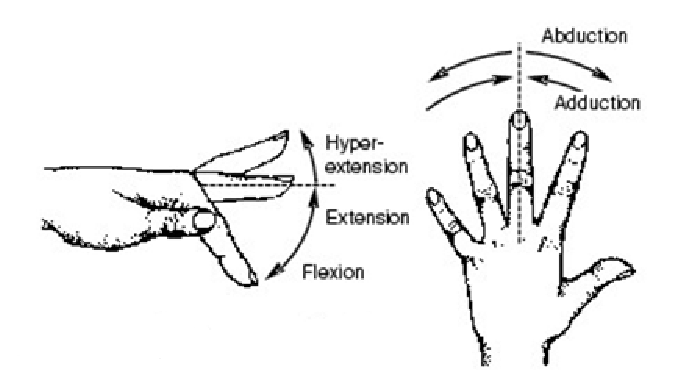
\includegraphics[width=7cm]{abduction}
\vspace{-20pt}
\caption{Hyperextension and Abduction}
\label{fig:hyperabduction}
\vspace{-10pt}
\end{figure}

\subsection{Finger Hyperextension}

\textbf{Hyperextension} (Figure \ref{fig:hyperabduction}) "\textit{puts more strain on the }[MCP] \textit{joints and tendons than the hand is accustomed to}" \cite{laviola1999survey} and therefore causes discomfort \cite{laviola1999survey}.
Even though this might seem redundant to the deviation from RRP on first sight, hyperextension takes a special position as it causes considerably more discomfort, compared to a full flexion of the fingers and compared to what the deviation from RRP would suggest.

For the \textbf{hyper extension} component \textbf{HE(x)} we simply summed up the the flexion/extension angle of the fingers MCP that had a negative angle and were therefore hyperextended.

\subsection{Finger Abduction}

Finger \textbf{abduction} (Figure \ref{fig:hyperabduction})
also causes stress on the MCP joint, the abduction muscles and tendons involved.

It was therefore also considered, analogue to the hyperextension, due to full abduction creating substantially more discomfort than full adduction.

We computed the \textbf{abduction} component \textbf{FA(x)} by adding up the absolute abduction/adduction angle for the finger. This is possible due to a fully adducted finger having an abduction angle of 0 in our model.


\subsection{Naive Metric}


Based on the model mentioned above\cite{vink2012editorial}, we then assigned the components to either comfort or discomfort. We then designed our metrics to be the added up component values \begin{math}(RRP, IFA, ...)\end{math} multiplied with weighting coefficients \begin{math}(c_{RRP(x)}, c_{IFA(x)}, ...)\end{math}. These weighting coeffitients were estimated for the \textbf{naive metric.} 
	\[
	Comfort(x) = c_{RRP}\cdot RRP(x)
	\]
	\[
	Discomfort(x) = c_{IFA}\cdot IFA(x)  +  c_{HE}\cdot HE(x)  +  c_{FA}\cdot FA(x)
	\]

The resulting metrics are expected to correlate with user perception, having the value 0 as maximum comfort and minimum discomfort respectively.


\subsection{Improved Metric}

Even though the naive metrics contain the causes of comfort and discomfort, they still lack deeper consideration for the anatomical differences between the fingers.
The concept of improvement extends the thought process already used for inter finger angles: instead of applying the metrics to the whole hand, have a look at the contributions from the individual fingers and weight them with importance coefficients. 

	\[
	Discomfort = c_{IFAindex}\cdot IFA(index)  +  c_{IFAmiddle}\cdot...
	\]

In our case we have 5 comfort values and a total of 12 discomfort values. 

However, the exact weighting coefficients are generally unknown and hard to estimate. To solve this problem, we reduced it to a curve fitting problem with 17 unknowns and used data, obtained from user evaluations to find the correct coefficients.

\section{Methodology}

For the collection of data, we created a test environment using \textbf{Unity 3D} with a total of two tasks. In the fist task, the subject would be shown a randomly generated hand posture on screen, using our naive metric to ensure a somehow homogenous distribution of expected comfort and discomfort. The subject was asked to mimic the hand posture with his or her dominant hand and afterwards rate the hand. As we did not expect the subjects to be familiar with current comfort and discomfort models, we asked them to rate hand postures on an intuitive scale ranging from 0 (very uncomfortable) to 10 (very comfortable). The subject was told to rate the hand posture with 0 points if he or she was unable to reproduce it. Before the actual evaluation subjects were shown two hand postures as a point of reference for comfort and discomfort. The first hand posture was a completely relaxed hand, the second hand posture was a randomly generated hand, that was challenging to mimic (Figure \ref{fig:Robot}).

In the second task, the subjects was again given a randomly generated hand posture. Again the subject had to mimic the hand posture with his dominant hand and give it a rating from 0 to 10. After confirming his or her rating, the subject had to perform a pointing task, more specifically a target shooting task (Figure \ref{fig:participant}). Therefore we tracked the subject's hand using an \textbf{ART Hand Tracking Device}, giving the subject a minimalistic representation of their hand position and indicating the forward direction of their hand with a rendered ray. The seated subject, with the elbow rested on a table, had to use this ray to aim down a total of 12 targets, appearing in random order, and shoot them, by pressing a button with the off-hand. By recording the hand posture before the trial using a Leap, and checking the hand posture during the test, we made sure that the user would not break the posture. 

\begin{figure}[h]
\centering
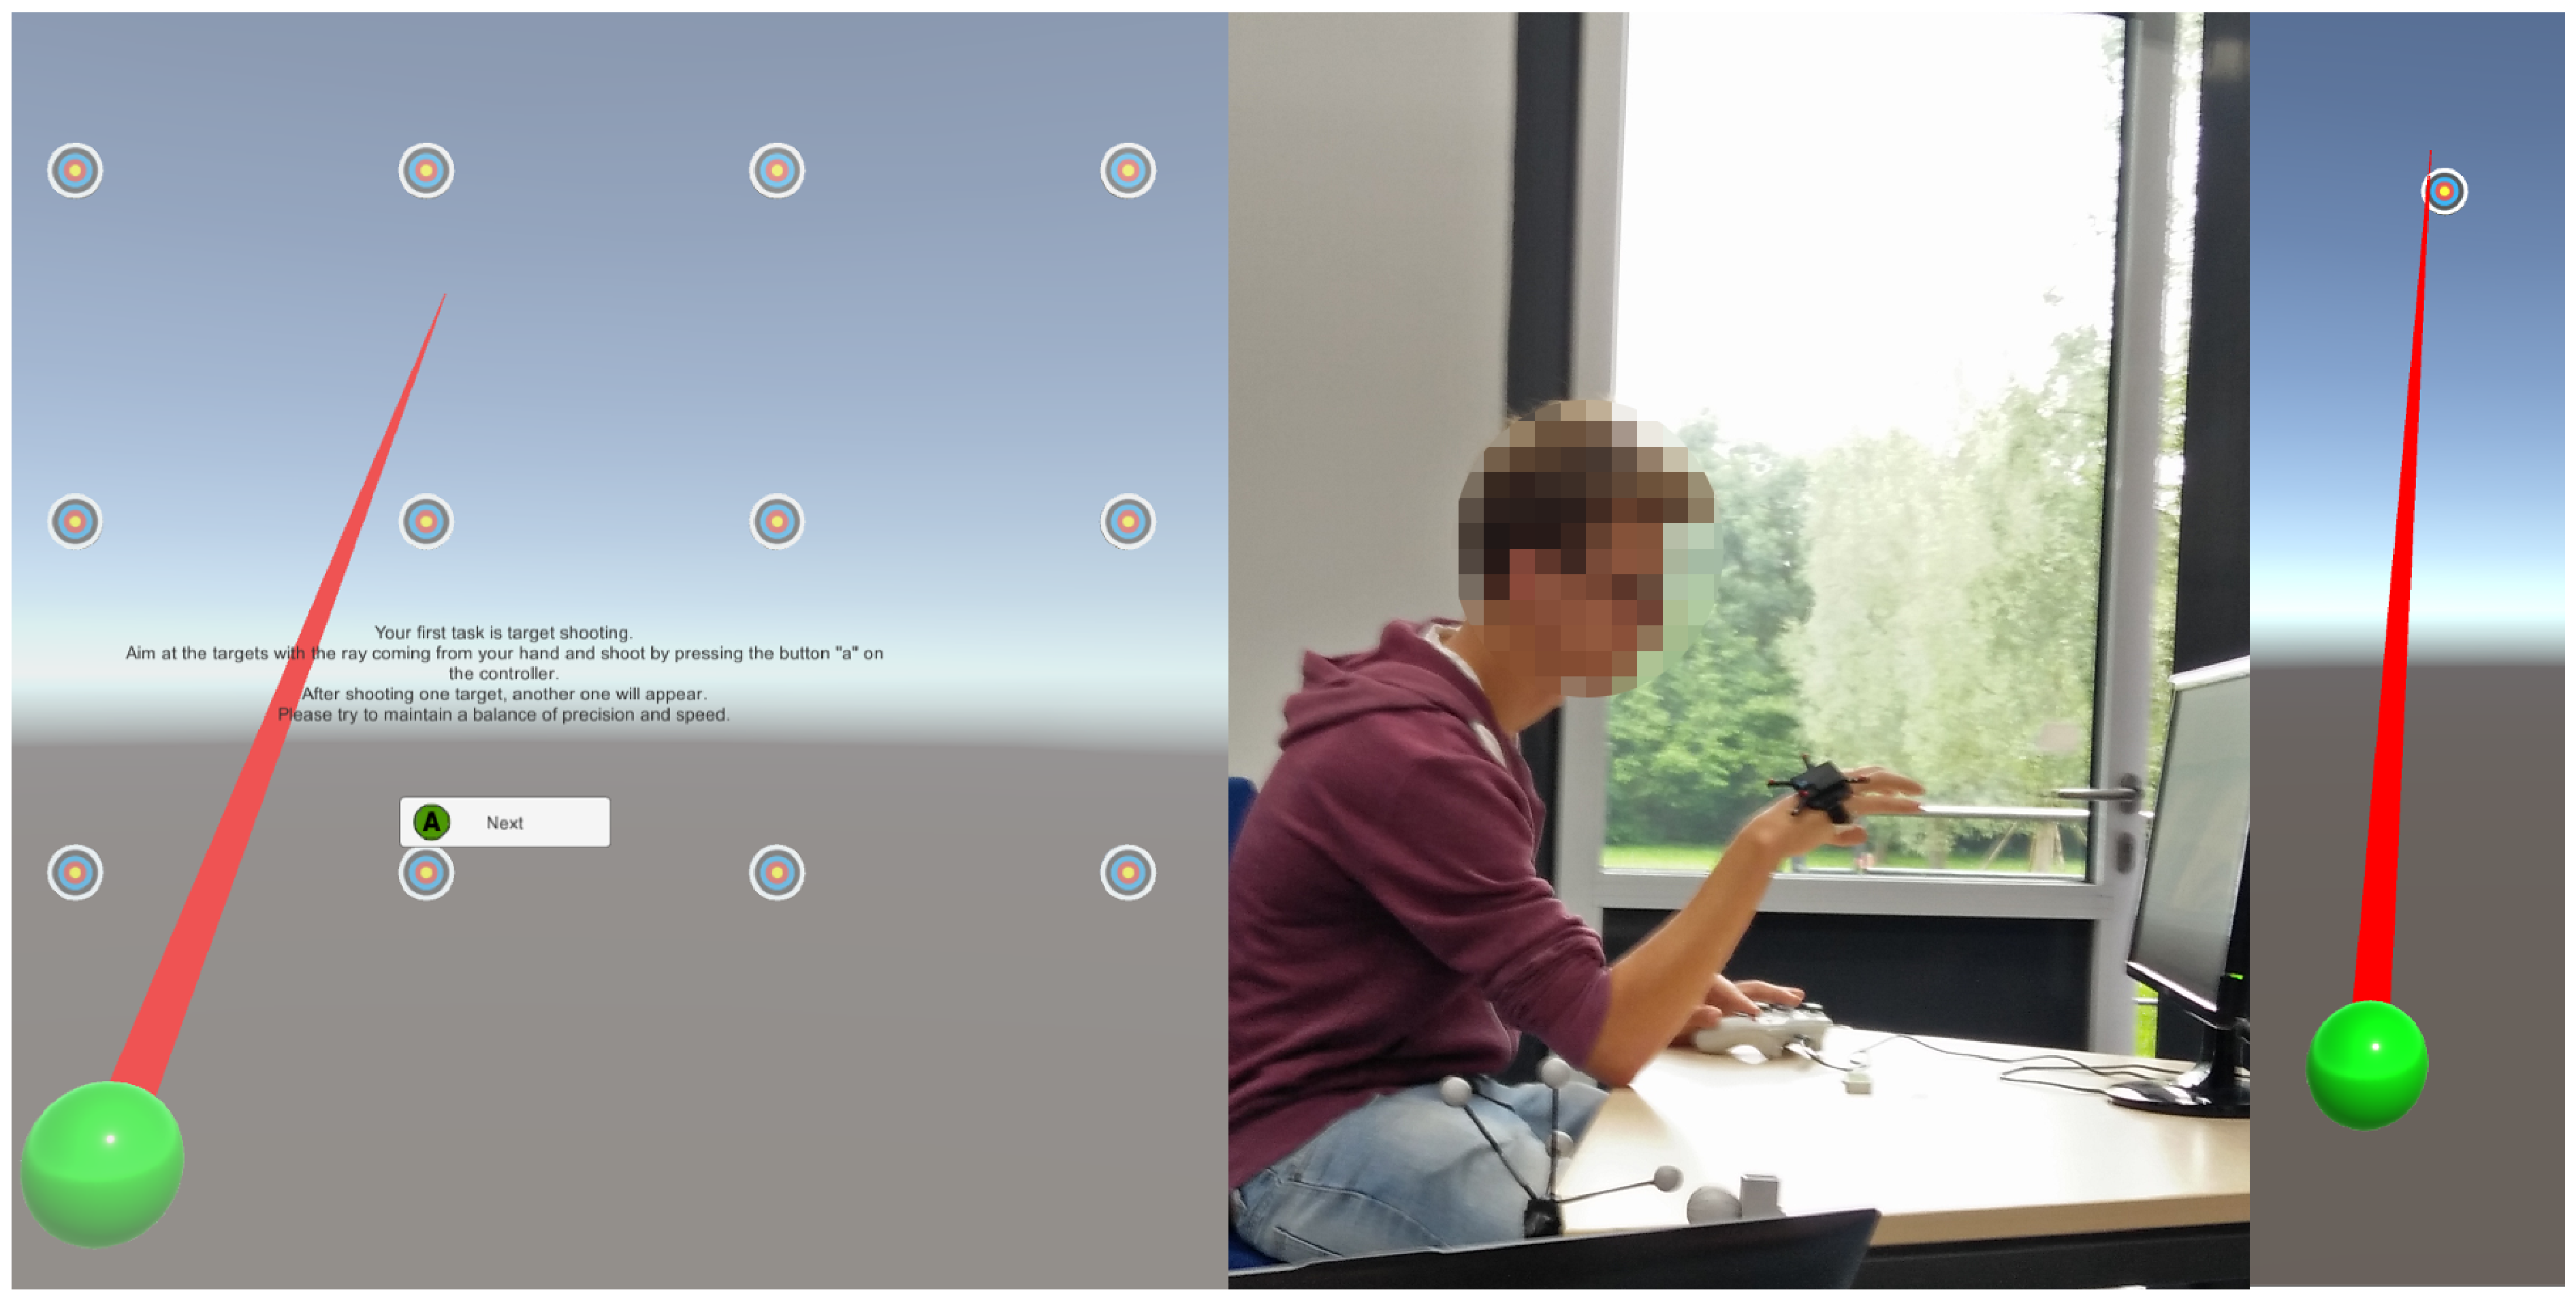
\includegraphics[width=8.45cm]{Participant}
\vspace{-20pt}
\caption{A Participant performing the Target Shooting (Best in Colour)}
\label{fig:participant}
\vspace{-10pt}
\end{figure}

As a metric for performance, we measured the total time taken for the test. In order to have this affected by precision, we made the targets rather small and told the subjects to perform the test as quickly as possible.

We conducted a total of two user studies involving 21 voluntary participants, that gained us 250 and 60 data sets for the metric and 35 data sets for the target shooting.
The subjects were informed about the aim of the study as well as their specific objectives beforehand.

As we expected both comfort and discomfort to affect performance and due to the users only giving us one value for comfort and discomfort, we decided to combine comfort and discomfort in our model as well. Finding the best fitting coefficients can be reduced to a curve fitting problem. Therefore we used the least squares algorithm on the first 250 data sets to fit the comfort/discomfort values to the user ratings. Afterward we tested our results against the remaining 60 data sets to check them for correctness. 

\section{Results \& Discussion}

\begin{table}[b]
\centering
\begin{tabular}{|c|c|c|} \hline
\#Figure & Correlation & p-value\\ \hline
\ref{fig:trainingData} & -0.6453242 & < 2.2e-16\\ \hline
\ref{fig:testData} & -0.748993 & 5.89e-12\\ \hline
\ref{fig:testDataNaive} & -0.6651999 & 6.73e-9\\ \hline
\ref{fig:targetShooting} & 0.4236101 & 0.01122\\ \hline
\end{tabular}
\caption{Pearson Correlations and P-values}
\label{tab:correlations}
\end{table}

\begin{figure}[b]
\centering
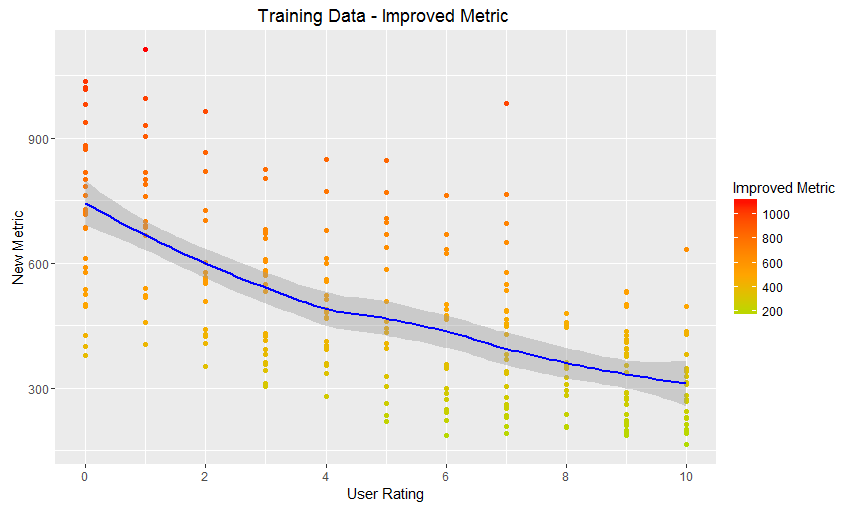
\includegraphics[width=8.45cm]{TrainingDataImproved}
\vspace{-20pt}
\caption{Improved Metric and User Rating in Training Data. \\
The Line Shows the Smoothed Conditional Mean, Calculated by the \texttt{geom\_smooth} Function in R.}
\label{fig:trainingData}
\vspace{-10pt}
\end{figure}

\begin{figure}[t]
\centering
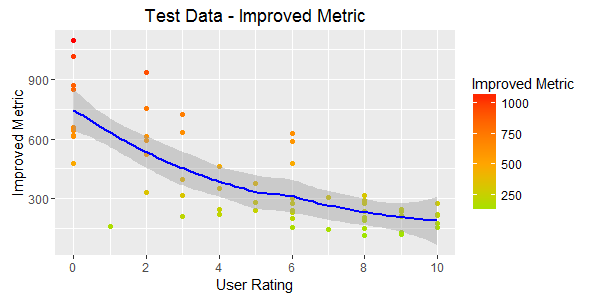
\includegraphics[width=8.45cm]{TestDataImproved}
\vspace{-20pt}
\caption{Improved Metric and User Rating in Test Data}
%\vspace{-5pt}
\label{fig:testData}

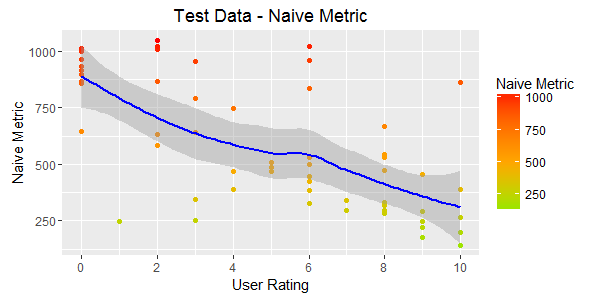
\includegraphics[width=8.45cm]{TestDataNaive}
\vspace{-20pt}
\caption{Naive Metric and User Rating in Test Data}
\label{fig:testDataNaive}
\vspace{-10pt}
\end{figure}


Unsurprisingly, there was a correlation in the training data between the user rating and our improved metric, generated using this data (Figure \ref{fig:trainingData}). However, the correlation found is still not perfect, having a value of approx. \textsl{-0,65} (Table \ref{tab:correlations}). For this we suspect multiple reasons: 

The participants most likely had differences in anatomy and set of mind, which caused them to subjectively rate comparable postures differently. In addition to that subjects had to give their rating after a relative short amount of time, therefore long time discomfort symptoms, like pain or cramping, might not have been experienced. Finally, the users could only rate the hands of continuous comfort/discomfort on a scale with 11 discrete steps, which probably created some additional error.

Even though the improved metric was created using a limited set of training data, it yielded a comparable correlation when applied to the test data (Figure \ref{fig:testData}). This indicates that the improved metric is a adequate extrapolation of the training data. Compared to the naive metric(Figure \ref{fig:testDataNaive}), there is only minor difference on first sight. However, the improved metric reduced the standard error, resulting in a better correlation and p-value (Table \ref{tab:correlations}).

\begin{figure}[h]
\centering
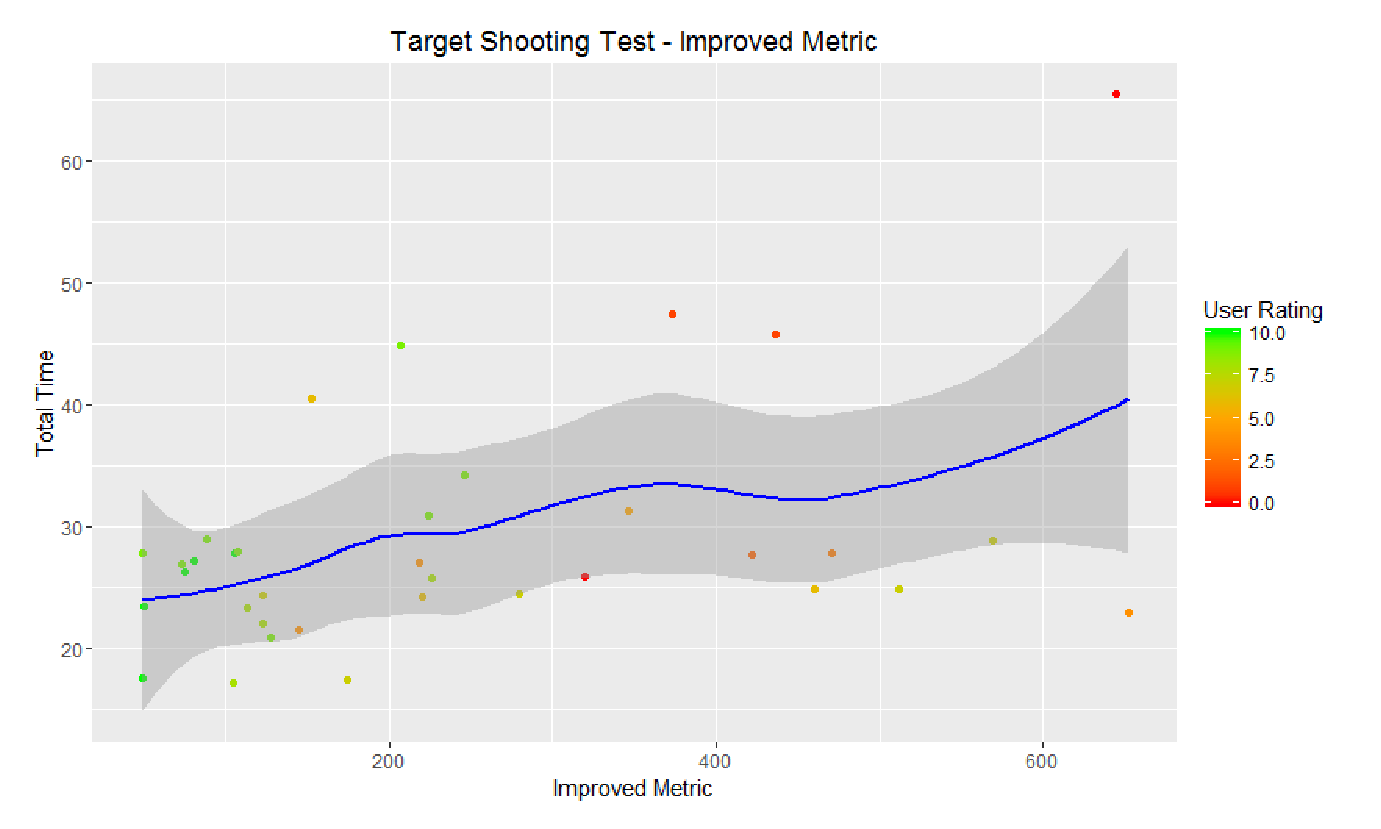
\includegraphics[width=8.45cm]{TargetShooting}
\vspace{-20pt}
\caption{Improved Metric Value and Total Task Time in Target Shooting}
\label{fig:targetShooting}
\vspace{-18pt}
\end{figure}

The results from the target shooting task (Figure \ref{fig:targetShooting}) indicate, that comfort and discomfort, as measured by our metric, do affect the performance and precision in context of hand postures. This strengthens the conclusion of Short et al. \cite{short1999precision}, that more comfortable postures generally create greater accuracy. However, the credibility of our results is limited by the relatively small dimensions of the user studies and more work and research will have to be done, in order to make strong conclusions.

Even though the results of this paper only apply to hand posture comfort/discomfort, the process of creating and testing a comfort/discomfort metric and its influence on performance/precision, as shown in this paper, can be transferred to other parts of the body. 

\section{Conclusion \& Future Work}

The main goal of this paper was to create a metric for quick and objective evaluation of hand posture comfort and discomfort. Furthermore we intended to demonstrate its relevance for design of hand postures, by proving its influence on precision and performance in a 3D pointing task. For the creation of the metrics we applied knowledge of the hand's anatomy and state of the art comfort and discomfort models and used data from a user study to improve the metric. Results from the testing user study suggest the improved metric to be a valid inference of the training data. In addition, the outcome of a small target shooting test indicate the existence of a correlation between comfort/discomfort and precision/performance, as already suggested for other contexts in other papers.

An important next step would be to take into account factors, neglected in this paper, for example long term effect of a hand posture on the perceived comfort and discomfort as well as on the performance and precision. Furthermore it would be helpful to determine other factors that might influence performance of a single hand task, to be able to find an optimum set of hand postures.
%\end{document}  % This is where a 'short' article might terminate

%
% The following two commands are all you need in the
% initial runs of your .tex file to
% produce the bibliography for the citations in your paper.
\bibliographystyle{abbrv}
\bibliography{handComfort}  % sigproc.bib is the name of the Bibliography in this case
% You must have a proper ".bib" file
%  and remember to run:
% latex bibtex latex latex
% to resolve all references
%
% ACM needs 'a single self-contained file'!
%
%APPENDICES are optional
%\balancecolumns

%\balancecolumns % GM June 2007
% That's all folks!
\end{document}
